\documentclass[a4paper,article,14pt]{extarticle}

% Подключаем главный пакет со всем необходимым
\usepackage{spbudiploma}
% Пакеты по желанию (самые распространенные)
% Хитрые мат. символы
\usepackage{euscript}
% Таблицы
\usepackage{longtable}
\usepackage{makecell}
\usepackage{threeparttable}
% Картинки (можно вставлять даже pdf)
\usepackage[pdftex]{graphicx}
\usepackage{wrapfig}
\usepackage[dvipsnames]{xcolor}
\usepackage{svg}
% Required package
\usepackage{tikz}
\usetikzlibrary{positioning}

\usepackage{amsthm,amssymb, amsmath}
\usepackage{textcomp}
\usepackage{enumitem}

\usepackage{minted} % для примеров кода (требует параметра -shell-escape)
\usemintedstyle{bw}


\begin{document}

% Титульник в файле titlepage.tex
\newgeometry{left=30mm, top=20mm, right=15mm, bottom=20mm, nohead, nofoot}
\begin{titlepage}
\begin{center}

\textbf{Санкт--Петербургский государственный университет}\\
\textbf{Факультет математики и компьютерных наук}


\vspace{35mm}

\textbf{\textit{\large Имя Отчество Фамилия}} \\[8mm]
% Название
\textbf{\large Выпускная квалификационная работа}\\[3mm]
\textbf{\textit{\large Тема работы: довольно длинное название\\строки на две минимум}}

\vspace{20mm}
Уровень образования: бакалавриат\\
Направление 01.03.02 «Прикладная математика и информатика»\\
Основная образовательная программа СВ.5005.2018
«Прикладная математика, фундаментальная информатика и программирование»\\
Профиль «Современное программирование»\\[25mm]


% Научный руководитель, рецензент
\begin{flushright}
\begin{minipage}[t]{0.65\textwidth}
{Научный руководитель:} \\
профессор, д.ф.-м.н. А.\,А.\,Выбегалло
\vspace{10mm}

{Рецензент:} \\
старший разработчик ООО <<Рога и копыта>>\\ А.\,И.\,Привалов
\end{minipage}
\end{flushright}

\vfill

{Санкт-Петербург}
\par{\the\year{} г.}
\end{center}
\end{titlepage}
\restoregeometry
\addtocounter{page}{1}


% Содержание
\tableofcontents
\pagebreak

\specialsection{Введение}

Введение широко представляет предметную область работы, указывает на место работы в научном или технологическом контексте.

\specialsection{Постановка задачи}
\textbf{Целью} моей выпускной работы является
создать расширяемый генератор учебных задач для курсов по обучению языкам программирования.

Основные задачи которые необходимо сделать:
\begin{enumerate}[label=\alph*.]
    \item Изучить существующие системы генерации случайных программ на предмет возможности их
          настройки и применимости результатов их работы в учебных целях.
    \item Создать систему
          генерации программ с возможностью настройки параметров для одного языка программирования (Python)
    \item Адаптировать систему к возможности поддержки других языков программирования.
\end{enumerate}

\textbf{Объектом} моего исследования являются инструменты генерации программного кода, а
\textbf{предметом} исследования --- применимость инструментов генерации код для создания учебных задач.

\section{Обзор и сравнение существующих генераторов программного кода}

\subsection{Понятие генерации программного кода}

\textbf{Генерация программного кода} --- это автоматическое создание программного кода специальным приложением, при котором по заданным условиям полностью или частично формируется исходный код программы. Такое специальное приложение называется \textbf{генератором кода}. Получается, что это программа, создающая программный код.

Основной сферой применения генераторов программного кода является автоматическое тестирования компиляторов. 
С помощью них можно обнаружить незаметные ошибки которые могут влиять на работу скомпилированного этими компиляторами программного обеспечения. В сравнение были включены
несколько инструментов для тестирования компиляторов.

Также для поиска существующих аналогов был произведен поиск в поисковых системах “Google” и “Google Scholar”
по следующим ключевым словам:
\begin{itemize}
    \item “C++ program generator”
    \item “program generator”
    \item “random program generator”
    \item "java program generator"
    \item "python program generator"
\end{itemize}

В обзор не включены различные генераторы привязок к SQL таблицам
(Spring Data JPA, jOOQ и подобные), шаблоны для языков разметки
(jinja, Django Template Engine) в виду их узкой специализации.
Были получены следующие результаты, соответствующие теме дипломной работы:
% Ненумерованная формула:

% \begin{equation}
%     \begin{pmatrix} \dot{\varphi}\\ \dot{\theta} \\ \dot{\psi} \end{pmatrix}
%     = \begin{pmatrix}
%         cos(\theta)cos(\psi) & -sin(\psi) & 0 \\
%         cos(\theta)sin(\psi) & cos(\psi)  & 0 \\
%         -sin(\theta)         & 0         &  1
%     \end{pmatrix}^{-1}
%     \begin{pmatrix} \omega_x\\ \omega_y \\ \omega_z \end{pmatrix}.
% \end{equation}

% Нумерованная формула:

% \begin{equation}
%     i^2 = -1.
%     \label{eq:my_ref}
% \end{equation}

% Тест ссылки на формулу \ref{eq:my_ref}.

\subsection{Automated C++ Program Generator using English Language Interface}

В статье \cite{pg-eli} описана программа, генерирующая код на C++ с помощью описания на английском языке.
Из описания выделяются ключевые слова и параметры, которым сопоставляются один из множества поддерживаемых шаблонов и алгоритмов, в которые передаются параметры.
Поддерживаются арифметические операции, числовые алгоритмы, строковые алгоритмы, алгоритмы над последовательностями и операции ввода-вывода.
% \begin{figure}[ht]
% \begin{center}
% \scalebox{0.4}{
%    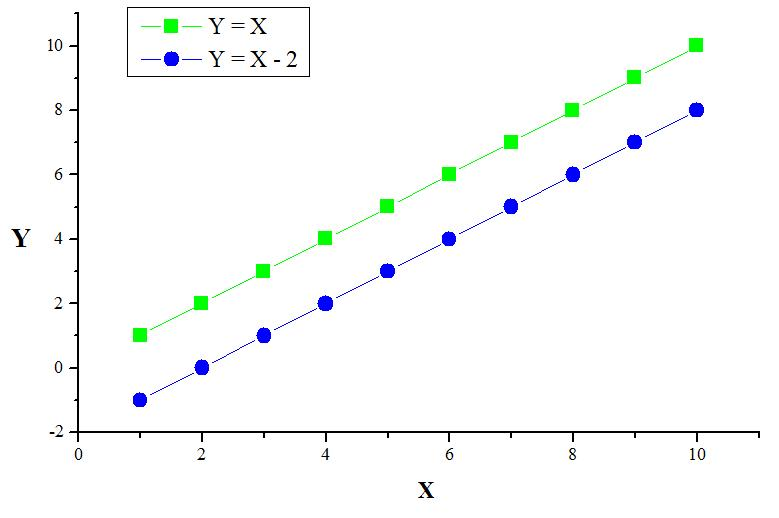
\includegraphics{images/graph.jpg}
% }

% \caption{
% \label{graph-fig}
%      Линейные функции.}
% \end {center}
% \end {figure}
% Ссылаемся на график~\ref{graph-fig}.

\subsection{Automatic code generation for C and C++ programming}

В статье \cite{acg-2021} описана программа, генерирующая код на C++ с помощью описания в виде блок-схем.
Элементами блок-схемы является ввод-вывод, условные ветвления и циклы.
Следствием этого является ограниченный набор поддерживаемых операций,
но в то же время за счет низкоуровневого интерфейса данная программа может генерировать более сложные программы.

\subsection{Csmith}

Csmith --- инструмент для генерации случайных программ на языке программирования C в соответствии со стандартом C99.
Используется в тестировании компиляторов, благодаря нему получилось найти более 400 ошибок в компиляторах языка C которые не были известны до этого.
Также поддерживает генерацию кода на C++. \cite{csmith}
% В работах иногда приводят фрагменты кода:
% 
% \begin{minted}{kotlin}
% fun main() {
%     val name = "stranger"
%     println("Hi, $name!")
%     print("Current count:")
%     for (i in 0..10) {
%         print(" $i")
%     }
% }
% \end{minted}


\subsection{Liveness-Driven Random Program Generation (ldrgen)}

Проект, основанный на идеях Csmith, также созданный для тестирования компиляторов.
Основная идея - уменьшение количества “мертвого кода” при генерации,
что позволяет добиться большего количества инструкций на строку кода и,
соответственно, генерировать более компактные программы для тестирования. \cite{ldrgen}


\subsection{Yarpgen}

Инструмент для генерации случайных программ на языке C для тестирования компиляторов.
Для тестирования вычисляется хэш всех значений глобальных переменных программы после ее запуска.
По сравнению с Csmith код, сгенерированный Yarpgen, более похож на написанный человеком,
так как в некоторых случаях сначала генерируется более высокоуровневая модель,
которая затем наполняется случайными данными.
Также гарантируется отсутствие неопределенного поведения у сгенерированных программ. \cite{yarpgen}

\subsection{Deepsmith}

Инструмент для генерации программ для библиотеки OpenCL на основе машинного обучения.
Сгенерированный код похож на написанный человеком так как модель обучена на open-source коде с github.
\cite{deepsmith}

\subsection{SL Random Program Generator}

Инструмент для генерации случайных программ на языке Python. Можно настраивать количество инструкций и используемые в выражениях операторы. 
Имеется веб-версия, гле также можно найти исходны код и грамматику. \cite{sl}

\subsection{Pyfuzz}

Инструмент для генерации случайных программ на языке Python. Используется для тестирования
инструментов компиляции и JIT-интерпретации Python-кода. \cite{pyfuzz}

Имеется веб-версия \cite{pyfuzz-web}

\subsection{Сравнительный анализ найденных инструментов и статей}

Сравнение аналогов будет проведено по следующим критериям:
\begin{itemize}
    \item “Читаемость кода”, то есть похож ли сгенерированный код на написанный человеком
    \item Возможность расширения на разные языки программирования (расширяемость)
    \item Наличие интерфейса для взаимодействия
    \item Возможность настройки параметров генерации
    \item Поддержка рандомизации, в частности, возможность настроить начальное значение для генератора случайных чисел
\end{itemize}

Для статей ответы критерии будут проверяться из описания, так как код реализации отсутствует в открытом доступе.

Сравнение по данным критериям представлено в Таблице \ref{table-smth}.

\begin{table}[ht]
\begin{threeparttable}[t]
\begin{tabular}{p{5.1em}|m{4em}m{5em}m{4em}m{4em}m{4em}}
    Инструмент                                                       & Чита-\newline емость & Расширя-\newline емость & Интер-\newline фейс & Настройка параметров & Рандо-\newline мизация \\
    \hline                                                                                                                                                                                  \\
    Automated C++ Program Generator using English Language Interface & +                    & +                       & Natural language    & +                    & -                      \\
    \hline                                                                                                                                                                                  \\
    Automatic code generation for C and C++ programming              & +                    & +                       & Block-scheme        & +                    & -                      \\
    \hline                                                                                                                                                                                  \\
    Csmith                                                           & -                    & -                       & CLI\tnote{1}                 & +                    & +                      \\
    \hline                                                                                                                                                                                  \\
    ldrgen                                                           & -                    & -                       & CLI                 & +                    & +                      \\
    \hline                                                                                                                                                                                  \\
    Yarpgen                                                          & -                    & -                       & CLI                 & +                    & +                      \\
    \hline                                                                                                                                                                                  \\
    Deepsmith                                                        & +                    & -                       & CLI                 & +                    & -                      \\
    \hline
    SL Random Program Generator & + & - & Web & + & +/-\tnote{2}   \\
    \hline
    Pyfuzz & - & - & Web and CLI & +\tnote{3}   & +\tnote{3}  \\
    \hline
\end{tabular}
\caption{
    \label{table-smth}
    Сравнение аналогов.}
\begin{tablenotes}
 \item[1] CLI = Command Line Interface (интерфейс командной строки)
 \item[2] Отсутствует возможность задания seed для генератора случайных значений.
 \item[3] Только в CLI
\end{tablenotes}
\end{threeparttable}
\end{table}
\clearpage

\subsubsection{Результаты сравнения}

Инструменты, описанные в статьях \cite{pg-eli} и \cite{acg-2021}, имеют разный интерфейс, но оба
имеют ограниченную параметризацию и генерируют читаемый код, однако не имеют поддержки рандомизации.

Csmith, ldrgen, и Yarpgen имеют схожий функционал и недостатки, однако среди них csmith имеет наиболее
широкую степень параметризации, Yarpgen и ldrgen имеют меньшую возможность кастомизации.

Deepsmith благодаря машинному обучению генерирует код, максимально схожий с написанным человеком,
однако, по этой же причине, обладает небольшой возможностью кастомизации и не поддерживает какую-либо
рандомизацию.

SL Random Program Generator имеет удобный веб-интерфейс, но ограниченную возможность
настройки и рандомизацию, так же очень ограничено количество поддерживаемых языковых конструкций языка Python.

Pyfuzz так же имеет веб интерфейс, однако в нем совсем отсутствует возможность настройки и рандомизации.
В CLI такая возможность присутствует, однако получившиеся программы все же используются для 
тестирования компиляторов и интерпретаторов, поэтому код получется плохо читаемым для человека.

\section{Разработка инструмента генерации программ}
Сравнительный анализ существующих решений для генерации программ показал, что
% * <Mark Zaslavskiy> 18:01:46 06 May 2022 UTC+0300:
% уточните - чем именно не подхдят
инструменты, используемые на практике, не подходят для учебных целей. Поэтому было принято решение
разработать собственную систему генерации программ для учебных задач.

\subsection{Требования к системе генерации}
Разрабатываемый инструмент должен обладать следующими возможностями:
\begin{itemize}
    \item Возможность генерации базовых элементов языка программирования;
    \item Поддержка генерации кода на разных языках, чтобы иметь возможность использовать данный
          инструмент в разных обучающих курсах;
    \item Расширяемость, что включает в себя:
          \begin{itemize}
              \item Гибкую систему создания шаблонов для генерации задач;
              \item Возможность настройки параметров генерации;
              \item Высокую вариативность задач, поддержку рандомизации отдельных элементов кода
          \end{itemize}
\end{itemize}

\subsection{Шаблоны программ}
\subsubsection{Общие единицы кода для разных языков}
\subsubsection{DSL}
\subsection{Примеры задач}


\section{Реализация инструмента генерации программ}

\subsection{Используемые технологии}
% * <Mark Zaslavskiy> 18:02:35 06 May 2022 UTC+0300:
% Сначала описывается архитектура, а затем детали реализации

Для разработки инструмента был выбран язык программирования Kotlin \cite{kotlin}. Это язык
программирования, разработанный компанией JetBrains в 2010 году. Основными
преимуществами этого языка программирования являются:
\begin{itemize}
    \item Кроссплатформенность
    \item Возможность интеграции с различными популярными системами сборки
          (Maven, Gradle, etc.)
    \item Возможность интеграции с java без переписывания имеющегося кода
\end{itemize}

Для сборки проекта использована система сборки Gradle \cite{gradle}.

В качестве системы контроля версия используется git, являющийся самой популярной системой
% * <Mark Zaslavskiy> 18:02:52 06 May 2022 UTC+0300:
% про выбор системы контроля и системы сборки писать не нужно
контроля версий на сегодня \cite{git}. Репозиторий с исходным кодом размещен на ресурсе Github
\cite{git} \cite{github} \cite{repo}.


\subsection{Архитектура системы}
Разработанная система имеет клиент-серверную архитектуру с отдельными микросервисами для
% * <Mark Zaslavskiy> 18:03:37 06 May 2022 UTC+0300:
% При описании архитектуры пишите, опираясь на цель и обосновывая ваши решения (просто так их констатировать - не очень) - почему клиент-серверная (как это поможет достижению цели)
некоторых компонент.

Клиентская часть представляет собой веб-сайт с помощью которого пользователь может делать
запросы на получение текста или картинки кода по шаблону (задаче). Также имеется возможность
делать запросы напрямую к API в формате JSON.

Серверная часть состоит из нескольких компонент: непосредственно веб-сервер, система генерации
кода и система проверки ответов студентов. В отдельный микросервис выделена система хранения
текстов и изображений программ, состоящая из базы данных, находящейся в изолированном окружении.

Для автоматизации развертывания системы генерации, поддерживания окружения для хранилища и
системы проверки используются технологии Docker \cite{docker} и docker-compose \cite{docker-compose}.
Благодаря Docker можно создать изолированное окружение (контейнер) для компонента, а docker-compose
позволяет объединять контейнеры в единую локальную сеть.
(\textit{TODO: описать для каких компонентов сделаны контейнеры})

Схема архитектуры показана на изображении \ref{architecture}, ниже подробнее описаны отдельные
компоненты.

\begin{figure}[ht]
    \begin{center}
        \scalebox{0.5}{
            \includesvg{images/architecture.svg}
        }
        \caption{\label{architecture} Архитектура системы генерации программ}
    \end{center}
\end{figure}
\clearpage



\subsection{Компоненты системы}
\subsubsection{Сервер}
Для компонента сервера было принято решение использовать библиотеку Ktor \cite{ktor}, так как
она позволяет быстро создать веб-сервер с нужным функционалом и имеет простой и элегантный API.
% * <Mark Zaslavskiy> 18:05:18 06 May 2022 UTC+0300:
% мне кажется, что надо найти более измеримые плюсы фреймоврка, нежели быстрота разработки (она больше про программиста) или элегантность :)
% ^ <Mark Zaslavskiy> 18:07:51 06 May 2022 UTC+0300:
% также по тексту - меняйте функционал -> функциональность

(\textit{TODO: описание методов API})

(\textit{TODO: примеры кода})

\subsubsection{Генерация}
Генерация IR (промежуточного представления программы, которое может затем
интерпретироваться в текст на разных языках) работает с помощью подстановки
параметров генерации (атрибутов) и \texttt{seed} для рандомизации в шаблон.

Генерация текста работает с помощью преобразования IR в текст с помощью
специальных классов - code mappers, которые отображают как общие, так и
специфические элементы IR в код. (\textit{TODO: примеры кода})

Генерация изображений реализована с помощью библиотеки \texttt{javax.imageio}
\cite{imageio}. По тексту генерируется изображение в формате jpeg.

\subsubsection{Хранилище сгенерированных программ}
% * <Mark Zaslavskiy> 18:05:47 06 May 2022 UTC+0300:
% опирайтесь на требования к решению - пишите, исполнению каких требований это поможет
Для поддержки работы с несколькими пользователями необходимо хранить сгенерированные
программы в базе данных. В базе хранятся параметры генерации, которые, вместе с
идентификатором задачи, выступают ключом. Значениями же являются текст и изображение
получившегося кода.

(\textit{TODO: примеры кода})

\subsubsection{Хранилище шаблонов}
Шаблоны задач хранятся в виде файлов на Kotlin, находящихся в отдельном модуле
проекта.


% !TEX root = ../main.tex


\section{Заключительный раздел с основными результатами}

\subsection{Подраздел}



\subsection{Подраздел}



% !TEX root = ../thesis-main.tex
\specialsection{Заключение}

Целью и основной задачей дипломной работы было создание генератора программ для обучения
программированию. В ходе выполнения работы были получены следующие результаты:

\begin{enumerate}
    \item Было проведено исследование существующих решений по генерации программ на
          предмет их применимости в обучающих целях. В ходе исследования были выявлены достоинства и
          недостатки имеющихся решений.
    \item Были сформулированы требования к генератору обучающих программ, учитывающие используемые
          модели в аналогах, их достоинства и недостатки. Из основных недостатков были выявлены: отсутствие возможности
          задать основную логику программы; малофункциональные модели задания шаблона кода при их
          наличии; отсутствие веб-интерфейса; отсутствие возможности хранения шаблонов и
          сгенерированных программ; отсутствие возможности генерации изображений.
    \item Создан предметно-ориентированный язык для описания задач (шаблонов кода), на основе которых генерируются примеры программ.
    \item Был реализован инструмент генерации программ, поддерживающий управление
          шаблонами кода, имеющий потенциал к расширению в сторону поддержки новых языков
          программирования, в настоящий момент поддерживающий генерацию кода на языке Python
          с помощью основных синтаксических конструкций.
\end{enumerate}

Таким образом, цель данной работы достигнута в полном объеме.

\bibliographystyle{unsrt} 
\bibliography{refs}
\end{document}